\subsection{Strategy Description}
Basing on the analysis and results of section 4 and 5, we are profoundly aware of the central role that Sources play in the whole Opioid Spread Model. Under the premises that the government management resources are limited, we hope to find an optimal strategy to maximize the control of opioid spread while minimize the government resources used. 

Therefore, the strategy we take should mainly focus on Sources. To be more specific, we plan to:
\begin{itemize}
	\item Sourcesforce the opioid investigation efforts in Source counties to decrease the amount of opioid storage $S(t)$.
	\item Intensify inspection and control of private vehicles passing through cross-county road, hoping to limit the amount of opioid transported from Sources to Consumers $T^{OUT}(t)$.
\end{itemize}

We make some adjustments on the existing Discrete Opioid Spread Model in order to simulate and quantify opioid spread. No additional information could reveal the precise relationship between  $S$ and $S'$. Intuitively, we assume that 
\begin{equation}
S'(t) = \delta S(t)
\end{equation}
where
\begin{equation}
\delta \sim U(0, 0.1)
\end{equation}

Corresponding to the strategy we proposed earlier, we add a storage control coefficient $\alpha$ and a transport control coefficient $\beta$, such that
\begin{comment}
\begin{equation}
\alpha S_i(t) - S_i'(t) = \lambda S_i(t) + \beta T_i^{OUT}(t), \alpha\in (0,1), \beta \in (1, +\infty)
\end{equation}
Combining (23-25), we have
\end{comment}
\begin{equation}
(1 - \lambda - \delta)\alpha S_i(t) = \beta T_i^{OUT}(t), \alpha\in (0,1), \beta \in (1, +\infty)
\end{equation}
We set $\alpha$ in a range of $(0,1)$ because we hope that the storage after control $\alpha S(t)$ is smaller than the original storage. Similarly, we set $\beta > 1$ in that an increase in $\beta$ causes a decrease in $T^{OUT}$ when the left side of the equation (28) is known.

Mathematically, we could combine $\alpha$ and $\beta$ into one parameter to simplify analysis:
\begin{equation}
\varphi = \frac{\alpha}{\beta}
\end{equation}
thus
\begin{equation}
 (1 - \lambda - \delta) \varphi S_i(t) = T_i^{OUT}(t), \varphi \in (0,1)
\end{equation}




To test the effectiveness of this strategy, we focus on how the change in $\alpha$ and $\beta$ influences storage.

\subsection{Evaluating the Strategy}
\subsubsection{Simulating Opioid Spread}

\begin{wrapfigure}[13]{r}{0.25\linewidth} % Inline image example
	\begin{center}
		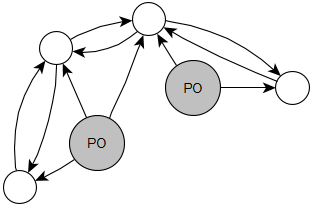
\includegraphics[width=\linewidth]{006}
	\end{center}
	\caption{Connection Between Sources and Others}
\end{wrapfigure}

We simulate opioid spread based on the directed graph we constructed in 4.2.1. We assume that drugs can be transported out of Sources into Consumers, but not vice versa. Thus we delete all edges pointing towards Sources in 4.2.1. 

We describe the simulation of opioid spread as:

\begin{enumerate}[(1)]
	\item At $t=0$, we initialize the diagram by setting the storage of Sources to $S_i(0)=\gamma_i$, where $\gamma_i>0$ is a constant for Source $i$. We construct set VISITED = $\emptyset$ and push all Sources into VISITED. We initialize an all-zero array S\_RECORD, with a mapping from node index to array index.
	
	\item At $t=k, k>0$, S\_RECORD is again set to zero and the storage of Sources to $S_i(0)=\gamma_i$. For all nodes in set VISITED, we calculate their opioid transportation to their out-neighbors using equation (9).For each node $i$, we add each $v_{ij}(t)$ to S\_Record[j]. After all nodes in the VISITED set were calculated, we add S\_Record[i] to $S_i$. After this, we traverse through the graph to add all nodes with $S>0$ but not yet in set VISITED into the set. 

\end{enumerate}

We compose a schematic diagram of storage flow. Inevitably, we will reach a point when all nodes are in the VISITED set. Simulation can carry on even when all nodes are visited. We visualize the spread in Figure 5:

\begin{figure}[H]
	\centering
	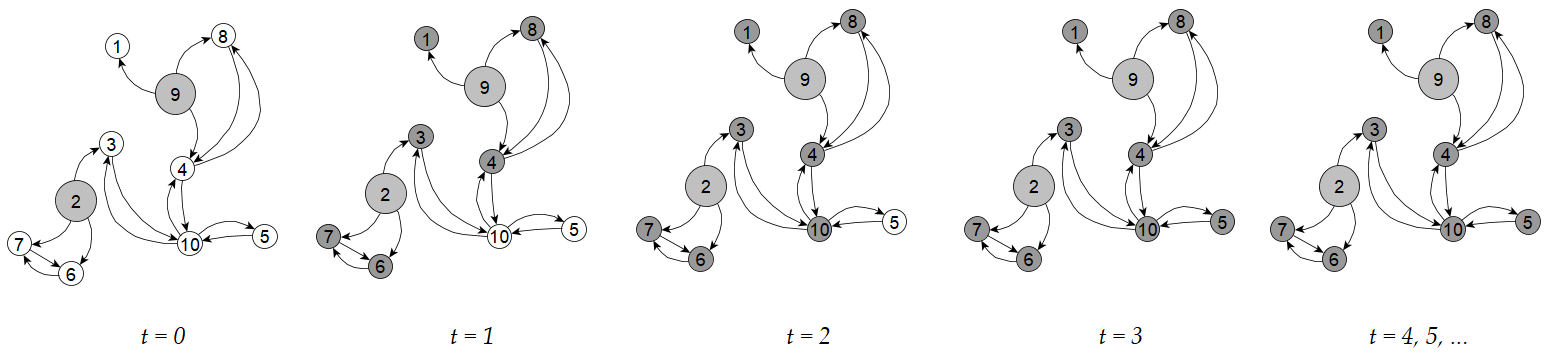
\includegraphics[width=\linewidth]{007}
	\caption{An Example Illustrating Opioid Spread Simulation. \textit{Node 2 and 9 are Sources. White nodes indiates nodes never visited. Gray nodes are nodes in VISITED set.}}
\end{figure}

We assume that in year 2017, we have reached a point where all nodes are visited. Therefore, we have only to consider the change in $S_i$ for each node $i$ with the increment of $t$. 

\subsubsection{Simulation Results}
We evaluate our strategy both qualitatively and quantatively. We take $\varphi = 0.4$ as an example.

Firstly, we compare the heatmap generated with that of non-control circumstances(i.e. $\varphi=1$). 

\begin{figure}[H]
	\centering
	\subfigure[$\varphi=1$]{
		\begin{minipage}[t]{0.45\linewidth}
			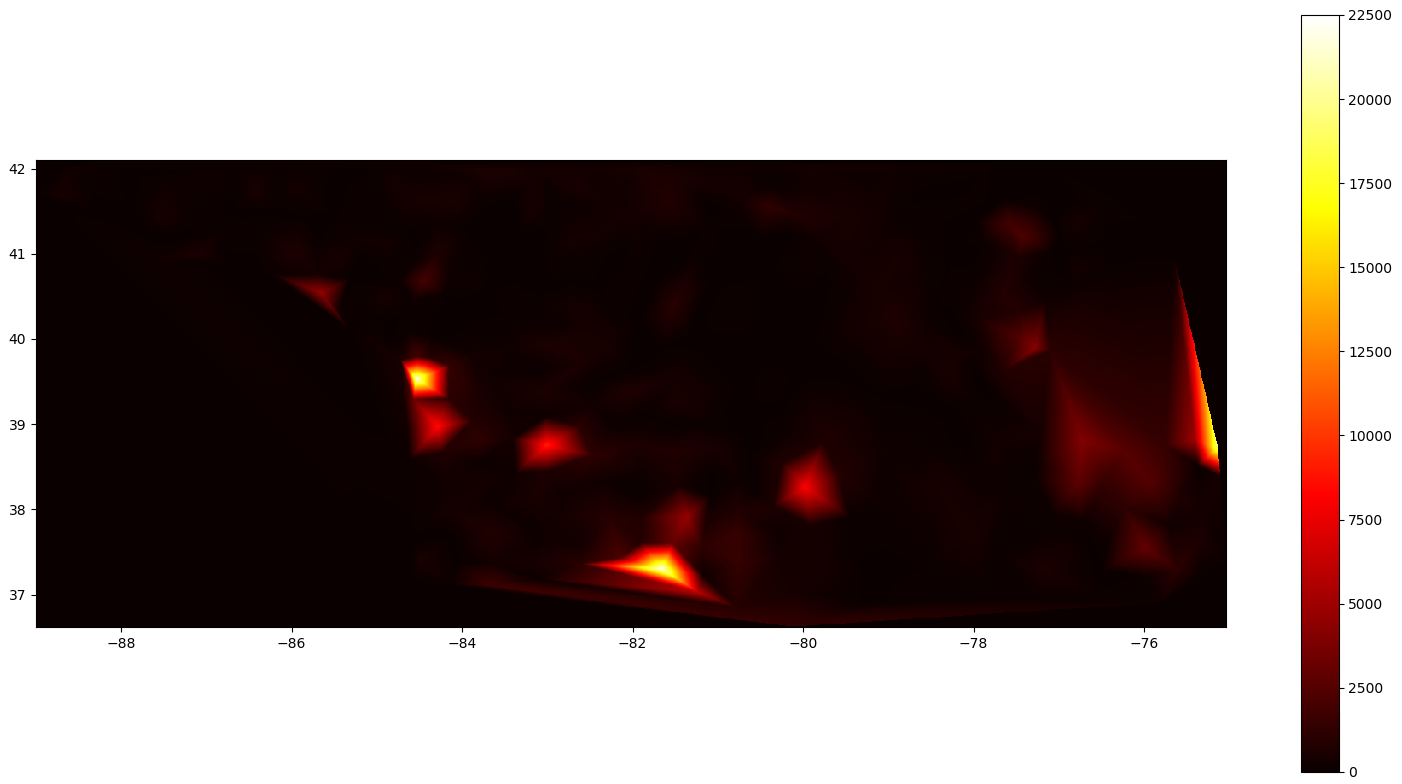
\includegraphics[width=\linewidth]{009}
		\end{minipage}
	}
	\subfigure[$\varphi=0.4$]{
		\begin{minipage}[t]{0.45\linewidth}
			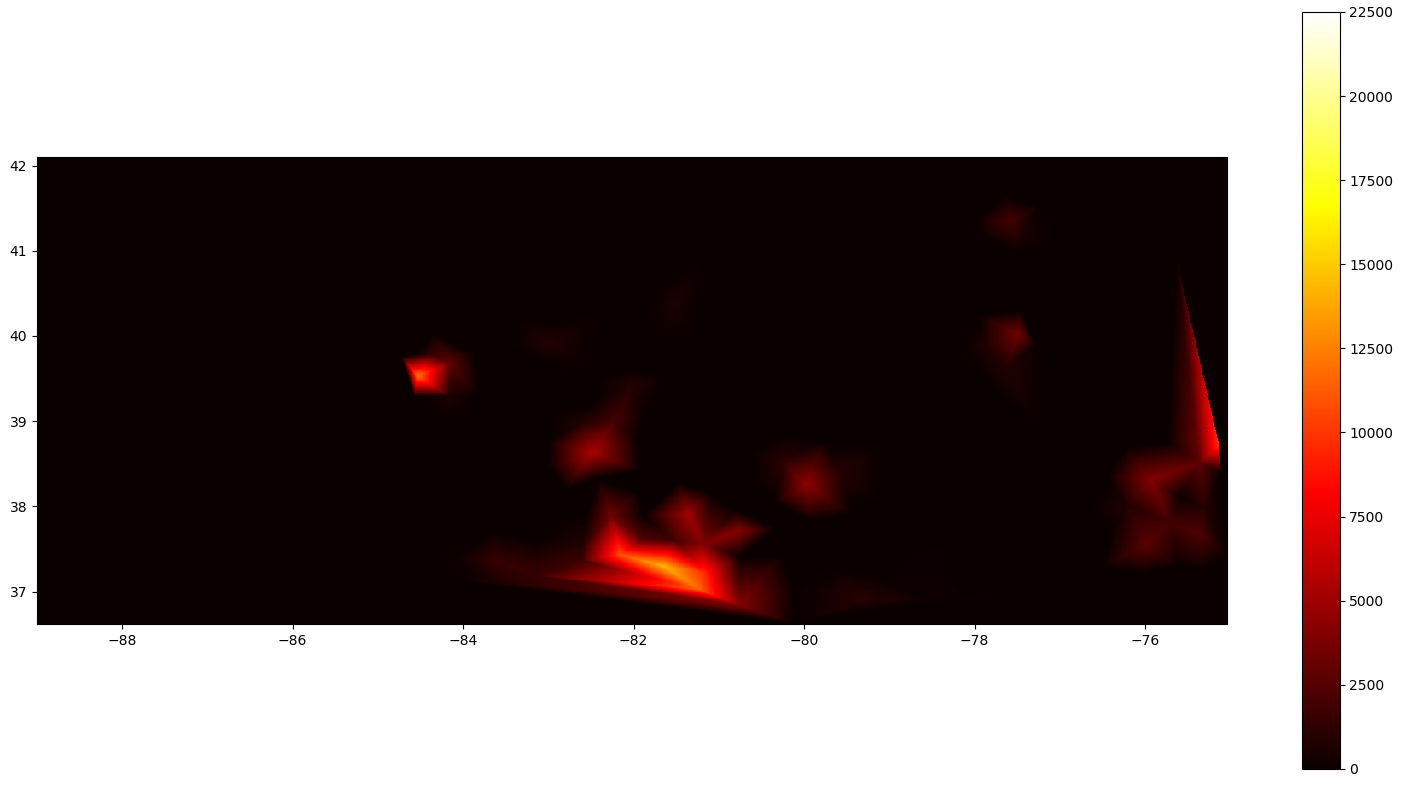
\includegraphics[width=\linewidth]{010}
		\end{minipage}
	}
	\caption{Heat Map Comparison}
\end{figure}
	
Secondly, let $n$ be the number of counties ranked second-level Sources and above. We compose a diagram of how $n$ changes over time. 

\begin{figure}[H]
	\centering
	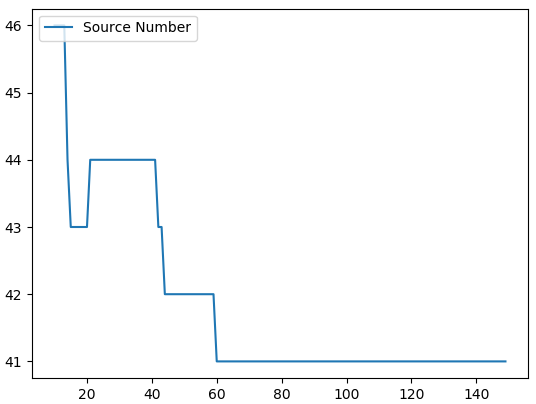
\includegraphics[width=0.3\linewidth]{011}
	\caption{n-t diagram}
\end{figure}

From the heatmap comparison(Figure 6), we reach the conclusion that the overall level of opioid storage declines dramatically. From the n-t Diagram(Figure 7), we can see that the number of Source counties decreased to some extent. 

%	\item Quantitative Method: using the threshold we proposed in Table Four, we hope that by controlling $\alpha$ and $\beta$, we could effectively reduce the number of first-level Sources and second-level Sources. Therefore, we define an ideal threshold $\mathcal{T}_1, \mathcal{T}_2$ to indicate an ideally low amount of first/second-level Sources, and compare how much time it takes for storage to change from the status in 2017 to our expected $\mathcal{T}_1, \mathcal{T}_2$ based on varying $\alpha$ and $\beta$. 
	
%	\item Qualitative Method: we generate a heat map of opioid storage at each time step $t$. Comparing these maps, we shall see the use-trend of opioids.


\subsection{Sensitivity Analysis: Identifing Significant Parameter Bounds}

We set simulation time long enough to observe how the number of Sources 
change over $\varphi$. As the scattered n-$\varphi$ diagram is shown below, the larger $\varphi$ is, the smaller $n$.

\begin{figure}[H]
	\centering
	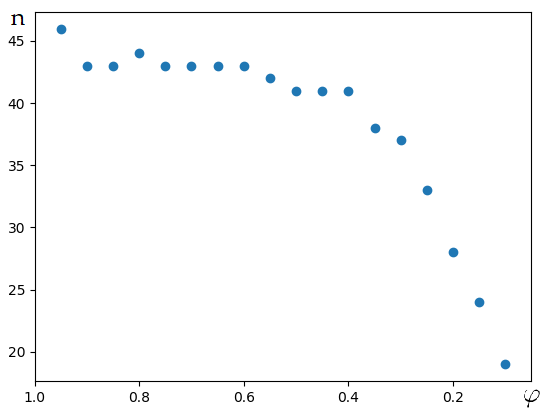
\includegraphics[width=0.3\linewidth]{008}
	\caption{n-$\varphi$ Diagram}
\end{figure}

From the diagram above, we observe that when $\varphi > 0.4$, the decrease in $n$ is relatively slow. However, a steep decrease occur when $\varphi < 0.4$. Thus, we suggest that the significant parameter(i.e. $\varphi$) bound is $0.4$.

\subsection{Extended Model}
To make the simulation of opioid spread closer to reality, we recommend some operations to improve the model, which are unnecessary in rough simulations.
\begin{enumerate}
	\item In our simulation process, we assume the Sources' storage $S(t)$ for each period $[t,t+1)$ to be a constant value. However, when control policies are functioning effectively, $S(t)$ is likely to be a gradually declining variable. We could define a decline coefficient to describe this scenario.
	
	\item Similar to what we analyzed for $S(t)$, when control strategies come into effect, the opioid consumption coefficient $\lambda$ would decline to some degree.
\end{enumerate}

However, we must keep in mind that a reasonable description of the declining process for the two coefficients stated above is no easy work.
